% Opcje klasy 'iithesis' opisane sa w komentarzach w pliku klasy. Za ich pomoca
% ustawia sie przede wszystkim jezyk i rodzaj (lic/inz/mgr) pracy, oraz czy na
% drugiej stronie pracy ma byc skladany wzor oswiadczenia o autorskim wykonaniu.
\documentclass[declaration,shortabstract,polish,lic]{iithesis}
\let\lll\relax
\usepackage{mathabx}
\usepackage[utf8]{inputenc}
\usepackage{fancyhdr}
\usepackage[toc]{appendix}
\usepackage{bookmark}
\usepackage{enumerate}
\usepackage{csvsimple}
\usepackage{float}

\usepackage{pdfpages}

\usepackage{color}
\definecolor{bluekeywords}{rgb}{0.13,0.13,1}
\definecolor{greencomments}{rgb}{0,0.5,0}
\definecolor{redstrings}{rgb}{0.9,0,0}

\definecolor{lightgray}{rgb}{.9,.9,.9}
\definecolor{darkgray}{rgb}{.4,.4,.4}
\definecolor{purple}{rgb}{0.65, 0.12, 0.82}

\usepackage{listings}


\pagestyle{fancy}
\fancyhf{}
\fancyfoot[CO,CE]{\thepage}
\fancyhead[RE]{\leftmark}
\fancyhead[LO]{\rightmark}
\renewcommand{\chaptermark}[1]{\markboth{Paweł Dybiec, Instytut Informatyki UWr}{}}
\renewcommand{\sectionmark}[1]{\markright{Weryfikacja możliwości sterowania łazikiem za pomocą sieci neuronowych}}

\polishtitle{Weryfikacja możliwości sterowania łazikiem za pomocą sieci neuronowych}
\englishtitle{TODO}

\author{Paweł Dybiec}
\advisor{dr Jan Chorowski}
\date{TODO} % Data zlozenia pracy
\transcriptnum{271900} % Numer indeksu
\advisorgen{dr Jana Chorowskiego} % Nazwisko promotora w dopelniaczu

\polishabstract{Sieci neuronowe są w stanie kierować samochodem na podstawie obrazu z
kamery\cite{nvidia}. Tematem tej pracy implementacja i przetestowanie autonomicznej jazdy
łazika Aleph 1 korzystającej z konwolucyjnych sieci neuronowych.}

\englishabstract{TODO ENG abstract}


\begin{document}
TODO: Zmienić kierunek na isim
\chapter{Preliminaria}
Ta praca została zrealizowana w ramach przedmiotu "Projekt: autonomiczna jazda łazikiem".
Z jego powodu(trzeba zmienic to wyrazenie), powstało wiele rozwiązań dla zadań z 
"konkursów łazikowych".

Żaden spośród łazików biorących udział w University Rover Challenge nie 
używa sieci neuronowych bezpośrednio do nawigacji , ale prawie wszystkie używają
ROS ( Robot Operating System ) jako podstawy całego oprogramowania. Z tego powodu
w tym rozdziale poruszone będą:
\begin{itemize}
  \item Podstawy sieci neuronowych.
  \item Architektura ROS
  \item Autonomia Aleph 1
\end{itemize}

\section{Podstawy sieci neuronowych}
\subsection{Jak działają}
\subsection{Jak trenować}
\subsection{Warstwy typowe dla CNN}
\subsection{Dlaczego działają}


\section{ROS}
Ros to otwarty system operacyjny przeznaczony dla robotów.
Dostarcza abstrakcję nad sprzętem oraz środki komunikacji między procesami.
Ze względu na modułową budowę oraz architekturę peer-to-peer procesy mogą
bezproblemowo działać na różnych komputerach.
\subsection{Node}
Podstawową jednostką w ROSie jest wierzchołek(node), jego głównym zdaniem jest
wykonywanie obliczeń. Wierzchołki razem tworzą graf, a komunikują się za 
pomocą tematów(topic).

Taka architektura (inspirowana budową mikrojądra) zapewnia lepsza ochronę na błędy
w porównaniu do architektury monolitycznej. Dodatkowo pojedyńczy element można
bezproblemowo przepisać, i to w innym języku.
\subsection{Topic}
Tematy(topic) pozwalają bezproblemowo zapewnić komunikację międzyprocesową
w ROSie. Każdy node może zadelkarować chęć nadawania bądź nasłuchiwania na
danym temacie. Przykładowo moduł jazdy autonomicznej może zasubskrybować
obraz z kamery Kinect, a publikować na temacie reprezentującym kierunek ruchu.
\subsection{Rosbag}
Rosbagi służą do zapisywania wybranych topiców wraz ze znacznikami czasu.
Niestety ten format wspiera tylko dostęp sekwencyjny przy odtwarzaniu, co wystarczy
do symulowania łazika, ale nie zawsze to wystarczyło. Aby temu zaradzić dane były
konwertowane do prostszego formatu.
%\subsection{Gotowe moduły}
%chyba nie aż tak ważne 
%tf,kamery,konwersje obrazków/strumieni

\section{Autonomia Aleph 1}
Co zostało zrobione na przedmiocie:
\begin{itemize}
  \item Sprzęt (mnóstwo)
  \item Mapa 3d (RTAB\_MAP)
  \item Rozpoznawanie klawiatur/piłek tenisowych
  \item Symulator
  \item kilka sieci obraz->kierownica
  \item wrappery/konwertery różnych protokołów/formatów
\end{itemize}

\chapter{Sieć pod symulator}
TODO: Rysunek sieci, obrazki aktywacji

\section{Dlaczego taka (a nie mniejsza)}
Dlaczego dropout

Dlaczego nieliniowe

Dlaczego tylko 1 dense

\section{Dane}
Jak długie przejazdy, i ile ich: 2 po 20 minut

Co gdyby zmniejszyć rozdzielczość ewaluowanych obrazkow do 16x8: jest ok

Jak wzbogacane: obrazy z 3 kamer + flip na środkowej


\chapter{Wyniki sieci}
Wytrenowana sieć potrafi przejechać zarówno cały tor na symulatorze, jak i
podziemny garaż instytutu. Na dodatek sieć trenowana pod symulator uczyła się
 jeździć tylko przeciwnie do ruchu wskazówek zegara. Po ustawieniu modelu w przeciwnym
kierunku, sieć potrafi bezproblemowo przejechać cały tor.

\section{Na co zwraca uwagę}
Aktywność sieci dla obrazków została wygenerowana za pomocą metody
Integrated Gradients\footnote{\href{https://arxiv.org/abs/1703.01365}{https://arxiv.org/abs/1703.01365}}.

Co było oczywiste w przypadku symulatora, sieć zwraca głównie uwagę na miejsca,
gdzie pojawiają się granice drogi \ref{sim_act}. Co ciekawe, reaguje też na ścianę
tworzącą horyzont, ponieważ zmienia wygląd w zależności od odległości i może
pomóc w orientacji (na trasie treningowej).
\begin{figure}
  \centering
  \fbox{
  \scalebox{0.5}{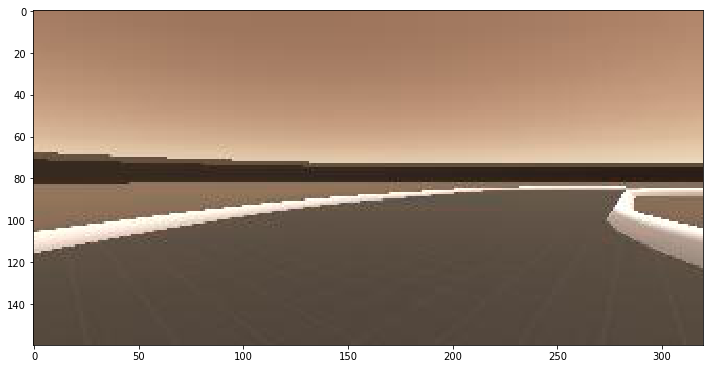
\includegraphics{img/sim_img.png}}
  }
  \caption{Obraz z symulatora}
  \label{sim_img}
\end{figure}
\begin{figure}
  \centering
  \fbox{
  \scalebox{0.5}{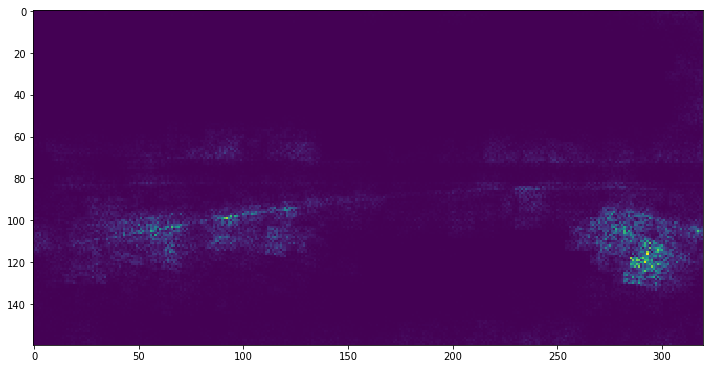
\includegraphics{img/sim_img_act.png}}
  }
  \caption{Na co sieć patrzy, symulator}
  \label{sim_act}
\end{figure}
\begin{figure}
  \centering
  \fbox{
  \scalebox{0.5}{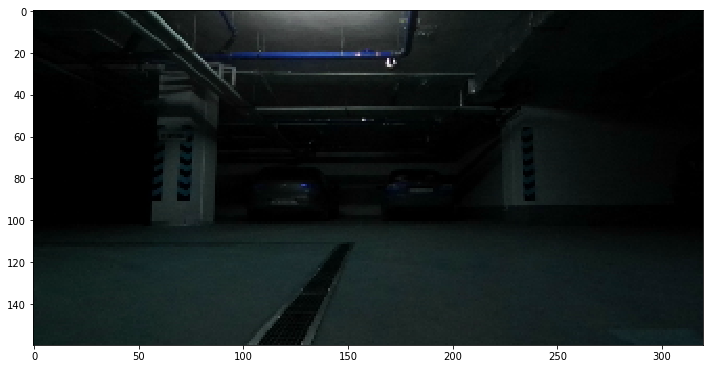
\includegraphics{img/real_img.png}}
  }
  \caption{Obraz z nagrania}
  \label{real_img}
\end{figure}
\begin{figure}
  \centering
  \fbox{
    \scalebox{0.5}{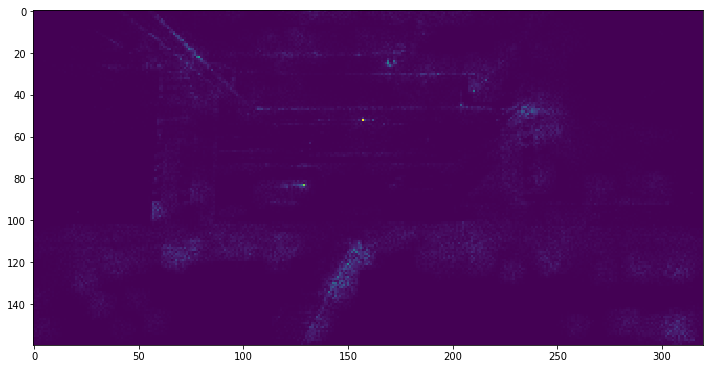
\includegraphics{img/real_img_act.png}}
  }
  \caption{Na co sieć patrzy, nagranie}
  \label{real_act}
\end{figure}

Z kolei dla łazika intensywność w najbardziej aktywnym miejscu jest dużo mniejsza \ref{real_act}.
Oznacza to, że nie sugeruje się tylko jednym obszarem z kamery. Najbardziej jednak 
zwraca uwagę na kratkę na podłodze, która mogłaby wystarczyć do nawigacji.

\section{W porównaniu do nagrania}
Na wykresie \ref{plot_ang} widać, że sieć (pomarańczowy kolor) mniej gwałtownie 
zmienia szybkość obrotu niż kierowca (kolor niebieski). Jednak sieć reaguje w podobnych momentach co kierowca na konieczność wykonania skrętu.

\begin{figure}
  \centering
  \fbox{
    \scalebox{0.5}{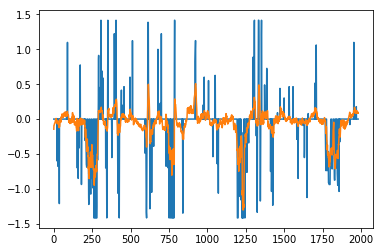
\includegraphics{img/real_data_ang.png}}
  }
  \caption{Prędkość obrotowa: sieć vs kierowca}
  \label{plot_ang}
\end{figure}

\section{Wpływ architektury}
W przypadku sieci pod symulator, usunięcie niektórych warstw konwolucyjnych
pozwalało modelowi nadal utrzymywać się na torze, natomiast taka sama zredukowana architektura 
nie radziła sobie dobrze w przypadku nagrań z prawdziwego łazika. Z kolei
usunięcie nieliniowości z warstw konwolucyjnych ograniczyło zdolności sieci do takiego stopnia,
że nie potrafiła się utrzymać na wirtualnym torze.

Usunięcie dropoutu bardzo szybko powodowało overfitting i sieć radziła sobie
dobrze tylko na danych uczących. Z kolei dodanie warstw liniowych na końcu nie 
poprawiało, ani nie pogorszało zbytnio wydajności sieci, przynajmniej dla
nagrań z symulatora. Na tej podstawie można wywnioskować, że większość interesujących 
cech obrazu została już znaleziona w ramach warstw konwolucyjnych, więc dla tak prostych danych zwiększenie modelu jest nieefektywne.

Co ciekawe, w przypadku wytrenowanego już modelu do symulatora zredukowanie 
rozdzielczości obrazów dziesięciokrotnie w każdym wymiarze (z rozdzielczości 
320x160 do 32x16),
i zwykłe przeskalowanie w górę przed zewaluowaniem wystarczy, żeby utrzymać się 
na torze.

Ponadto, sieć uczona na obrazie kolorowym działa bezproblemowo, gdy
zredukuje się obraz do skali szarości. Jedyne, co należy wykonać to stworzyć obraz kolorowy, w którym każdy z kanałów RGB będzie powtórzonym obrazem wejściowym.


\chapter{Co dalej}
Najprostszym następnym krokiem jest zwiększenie danych o dodatkowy wymiar, i nauczenie takiej
sieci decyzji na podstawie $k$ (niekoniecznie) ostatnich zdjęć. Innym prostym rozwiązaniem,
które można z tym połączyć jest zmiana perspektywy kamery na zdjęcie z góry.

Bardziej ambitnym pomysłem jest wytrenowanie rekurencyjnej sieci neuronowej (RNN),
gdyby ją dobrze nauczyć sama wyciągnie kontekst. Ale problemem przy jej trenowaniu
będzie fakt, że prostą strategią dla takiej sieci jest powtarzanie ostatniego wypisanego
wyniku, a to dlatego że prędkość jest ciągła.

Kolejnym rozwiązaniem jest reinforced learning, sieć karało by się za
każdą interwencję lub wyjechanie poza trasę. Niestety problemem tutaj jest 
fakt, że jak błąd prawdziwego pojazdu może być kosztowny lub niebezpieczny.

Oczywiście pozostają też rozwiązania nie używające sieci neuronowych, można
przykładowo stworzyć program pilnujący aby łazik nie wjechał w przeszkodę.




\begin{thebibliography}{1}
\bibitem{test} autor \href{https://example.com}{Tytuł}, 2018
\bibitem{nvidia} Mariusz Bojarski and
               Davide Del Testa and
               Daniel Dworakowski and
               Bernhard Firner and
               Beat Flepp and
               Prasoon Goyal and
               Lawrence D. Jackel and
               Mathew Monfort and
               Urs Muller and
               Jiakai Zhang and
               Xin Zhang and
               Jake Zhao and
               Karol Zieba \href{https://arxiv.org/abs/1604.07316}{End to End Learning for Self-Driving Cars}


\end{thebibliography}
\renewcommand\appendixtocname{Dodatki}
\bookmarksetupnext{level=part}
\begin{appendices}
\addtocontents{toc}{\protect\setcounter{tocdepth}{1}}
\makeatletter
\addtocontents{toc}{
  \begingroup
  \let\protect\l@chapter\protect\l@section
  \let\protect\l@section\protect\l@subsection
}
\makeatother
  \chapter{Instrukcja ruchomienie symulatora i sieci}
TODO: przepisać z repo

\addtocontents{toc}{\endgroup}
\end{appendices}

\end{document}
